\chapter{Background}\label{chp:bckgrnd}

\section{Electronic Structure Calculations}
Electronic structure methods have become an essential tool in materials science over the last three decades. Any relevant physical property of real materials can, in principle, be described by the laws of quantum mechanics. The foundation of these methods is the approximate solution of the many-body Schr\"odinger equation. Given the positions of the atomic nuclei and the total number of electrons in the system, the energy and other properties can be approximated. The ability to obtain a solution that is good enough requires an efficient description of the electronic system and considerable  computational power.



\subsection{The Many-Body Hamiltonian}
The quantum theory of electrons and nuclei controls the characteristics of matter over wide ranges of temperature and pressure. One of the most fundamental qualities of solids is that they have a variety of properties that result from the collective behavior of atoms. Electrical conductivity as well as magnetism arise as collective properties of the atoms in the solid. The wavefunction of the solid can be described by the Schr\"odinger equation,
\begin{equation}
	\mathcal{H}\ket{\Psi(t)} = i\hbar  \frac{\partial}{\partial t}\ket{\Psi(t)},
\end{equation}
where $\mathcal{H}$ is the Hamiltonian operator. If the Hamiltonian is time-independent, the Schr\"odinger equation can be simplified. For time-dependent problems, the wavefunction can be broken into the product of a time-dependent part and a time-independent part, the latter of which depends on the positions of the electrons and nuclei. The solution of the time-dependent Schr\"odinger equation is of the following form:\footnotemark
\footnotetext{More precisely, the solution would be written as the superposition $\Psi(\vb{r},t) = \sum_j C_j \psi_j (\vb{r}) e^{-iE_jt/\hbar}$, where $\psi_j(\vb{r})$ are eigenfunctions of the time-independent Schr\"odinger equation and $C_j$ are complex coefficients.} 
\begin{equation}
\ket{\Psi(\vb{r},t)} = e^{-iEt/\hbar}\ket{\psi(\vb{r})}
\end{equation}
The time-dependent part is trivial. The time-independent part obeys the time-dependent Schr\"odinger equation,
\nomenclature{$\mathcal{H}$}{many-body Hamiltonian}
\nomenclature{$\Psi$}{wavefunction}
\nomenclature{$Z_a$}{charge of $a$\textsuperscript{th} nucleus}
\begin{equation}\label{sheqn}
	\mathcal{H}\ket{\psi_j} = E_j\ket{\psi_j},
\end{equation}
where the Hamiltonian operator represents the total energy of the particles:
\begin{align}\label{hameqn}
 \mathcal{H} &= -\sum_j \frac{\hbar^2}{2m_e}\nabla^2_j - \sum_a \frac{\hbar^2}{2M_a}\nabla^2_a \nonumber \\
			& \quad -\sum_{j,a}\frac{Z_ae^2}{\abs{\vb{r}_j-\vb{R}_a}} + \frac{1}{2}\sum_{j,k}^{j\neq k} \frac{e^2}{\abs{\vb{r}_j - \vb{r}_k}} + \frac{1}{2}\sum_{a,b}^{a\neq b} \frac{Z_aZ_be^2}{\abs{\vb{R}_a - \vb{R}_b}} \nonumber \\
 \mathcal{H} & \stackrel{\text{(atomic unit)}}{=} -\sum_j\frac{1}{2}\nabla^2_j - \sum_a\frac{1}{2\tilde{M}_a}\nabla_a^2 \nonumber \\
			& \quad -\sum_{j,a}\frac{Z_a}{\abs{\vb{r}_j - \vb{R}_a}} + \frac{1}{2}\sum_{j,k}^{j\neq k} \frac{1}{\abs{\vb{r}_j-\vb{r}_k}} + \frac{1}{2}\sum_{a,b}^{a\neq b} \frac{Z_aZ_b}{\abs{\vb{R}_a - \vb{R}_b}} \nonumber \\
   & = T_e + T_N + V_{Ne}(\vb{r},\vb{R}) + V_{ee}(\vb{r}) + V_{NN}(\vb{R}) 
\end{align}

\nomenclature{$m_e$}{mass of a single electron}
\nomenclature{$\vb{r}_j$}{position of $j$\textsuperscript{th} electron}
\nomenclature{$\vb{R}_a$}{position of $a$\textsuperscript{th} nucleus}
It is convenient to use atomic units~(see Appendix~\ref{appen_atomicunit}), which will be used for the remainder of the discussion. In these units, the electron mass $m_e$ as well as the elementary charge $e$, the reduced Planck constant $\hbar$, and Coulomb's constant $1/4\pi\epsilon_0$ are unity, leaving $\tilde{M}_a = M_a/m_e$ as the relative atomic mass of the nucleus of atom $a$. $\vb{r}_j$ denotes the position of the $j$\textsuperscript{th} electron, while $\vb{R}_a$ is the position of the nucleus of atom $a$ and $Z_a$ is that nucleus' atomic number. A solution of the time-independent Schr\"odinger equation~\eqref{sheqn} would be a function dependent on the spatial coordinates of all particles in the system and is, as such, only obtainable for very idealized systems. The Schr\"odinger equation with the above Hamiltonian is impossible to solve exactly for most of systems of interest. A series of approximations and methods were therefore developed to reduce the complexity of the problem. With the help of Eqn.~\eqref{hameqn} the Schr\"odinger equation \eqref{sheqn} becomes 

\begin{equation}
 [T_e + T_N + V_{Ne}(\vb{r},\vb{R}) + V_{ee}(\vb{r}) + V_{NN}(\vb{R})]\Phi(\vb{r},\vb{R}) = E\Phi(\vb{r},\vb{R})
\end{equation}
In order to simplify the equations, the electronic coordinates and spin indices are combined into a vector $\vb{r} = (\vec{r},s)$, and $\vb{R}$ denotes the nuclear coordinates. The wavefunction here is a regular function of the atomic positions but a quantum state $\ket{\Phi(\vec{r})}$ in the Hilbert space for the electrons and nuclei, so that \mbox{$\Phi(\vec{r}) = \braket{\vec{r}}{\Phi(\vb{r},\vb{R})}$}. The nuclear mass exceeds the electron mass by more than three orders of magnitude, and so the electrons and nuclei move on different time scales. Thus, the wavefunction $\Phi(\vb{r},\vb{R})$ can be separated into an electronic part $\Psi(\vb{r},\vb{R})$ and a nuclear wavefunction $\chi(\vb{R})$,
\begin{equation}
\Phi(\vb{r},\vb{R}) = \Psi(\vb{r},\vb{R})\chi(\vb{R})
\end{equation}
The nuclear wavefunction is much more localized, which is why the Schr\"odinger equation can be separated into two parts:
\begin{align}
[T_e + V_{ee}(\vb{r}) + V_{Ne}(\vb{r},\vb{R})]\Psi(\vb{r},\vb{R}) & = \epsilon_n(\vb{R})\Psi(\vb{r},{R})\label{bo1} \\
[T_N + V_{NN}(\vb{R}) + \epsilon_n(\vb{R})]\chi(\vb{r}) & = E\chi(\vb{R})\label{bo2}
\end{align}
The nuclear positions $(\vb{R})$ in the equation~\eqref{bo1} serves only as a parameter and it is possible to use the \textit{adiabatic} or \textit{Born--Oppenheimer} approximation. On the timescale of the nuclear motion, the electron follow the ions adiabatically. As a further approximation, the quantum effects on the motion of the nuclei are neglected and the time-dependent Schr\"odinger equation is replaced by Newton's equation of motion;
\begin{align}
\frac{\partial P_I}{\partial t} & = -\nabla_I E_0 (\vb{R}) \\
\text{with} \quad E_0(\vb{R}) & = \epsilon_0(\vb{R}) + V_{NN}(\vb{R})
\end{align}
This refers to so-called \textit{ab-initio} molecular dynamics, where the forces around a nuclei are calculated from the electronic ground state. Here, $P_I$ is the momenta of the nucleus.
\nomenclature{$P_I$}{momentum of the $I$\textsuperscript{th} nucleus}
Equations~\eqref{bo1} and \eqref{bo2} are not generally applicable. However, for several physical systems, the Born--Oppenheimer approximation works and Eqn.~\eqref{bo1}, \eqref{bo2} produces meaningful results. In solid state physics, Eqn.~\eqref{bo2} is usually written in a classical form and Eqn.~\eqref{bo1} becomes the problem to be solved. It is still a very complicated equation, where the term describing the interaction between electrons would require the knowledge of $d^{3N}$ ($d$= number of discrete points) variables for a system of $N$ electrons. Such a large number of variables make the problem computationally not tractable and several approximate methods have been developed. Some of the important methods will be discussed in the next of this chapter.

These approximate methods are based on the \textit{independent particle} approximation, in which the Hamiltonian takes the form
\begin{equation}
	\mathcal{H} = \sum_j \mathcal{H}_j.
\end{equation}
The electronic wavefunction can be written as the product of single-particle wavefunctions. This leads to a further simplification of the Hamiltonian,
\begin{align}\label{ham1}
	\mathcal{H} &  = -\sum_j^N \frac{1}{2}\nabla^2_j - \sum_j^N\sum_a^M \frac{Z_a}{\abs{\vb{r}_j - \vb{R}_a}} + \frac{1}{2}\sum^N_{j\neq k}\sum^N_k\frac{1}{\abs{\vb{r}_j - \vb{r}_k}} \nonumber \\ 
	 &\quad  = T_e + V^{\text{ext}} + \frac{1}{2}\sum_{j\neq k} \upsilon_{jk}\Big(\abs{\vb{r}_j - \vb{r}_k}\Big) .
\end{align}



\subsection{Hartree--Fock Approach}
A very simple way to write the many-electron wavefunction is as a product of single-particle wavefunctions:
\begin{equation}\label{hwf}
\Psi(r_1,r_2,\dots,r_N) = \prod_j^N \psi_j(r_j).
\end{equation}
The Hamiltonian \eqref{ham1} is not just a sum of single-particle Hamiltonians: the true wavefunctions cannot be written in the product of the form \eqref{hwf}. Furthermore, the wavefunction in~\eqref{hwf} does not have the \textit{antisymmetry} property required for fermions.

The fermionic nature of the electrons imposes the Pauli exclusion principle as an additional constraint. One can achieve an antisymmetric many-body wavefunction by writing the electronic wavefunction as a Slater determinant of single-particle wavefunctions:
\begin{equation}\label{hfwf}
\Psi(r_1,r_2,\dots,r_N) = \frac{1}{\sqrt{N!}}\begin{vmatrix}
\psi_1(\vb{r}_1) & \psi_1(\vb{r}_2) & \dots & \psi_1(\vb{r}_N) \\
\psi_2(\vb{r}_2) & \psi_2(\vb{r}_2) & \dots &  \dots			\\
\vdots			 &					& \ddots &					\\
\psi_N(\vb{r}_1) & \dots			&		 &  \psi_N(\vb{r}_N) 
\end{vmatrix}.
\end{equation}
The expectation value of the Hamiltonian~\eqref{ham1} can be calculated using this wavefunction, which leads to an energy functional that can be minimized variationally~\eqref{vareqn}. 
\begin{equation}\label{vareqn}
E \le E' \equiv \frac{\bra{\Psi}\mathcal{H}\ket{\Psi}}{\braket{\Psi}{\Psi}} 
\end{equation}
Here, any state $\ket{\Psi}$ provides an upper bound $E'$ for the exact ground-state energy $E$. An additional constraints is that the single-particle orbitals are to be normalized. The normalization condition is
\begin{equation}\label{norm1}
\braket{\psi_i(\vb{r}_i)}{\psi_j(\vb{r}_j)} = \int \psi_i(\vb{r})^{\ast} \psi_j(\vb{r})d\vb{r} = \delta_{ij}.
\end{equation}
The many-particle wavefunction~\eqref{hfwf} and the Hamiltonian~\eqref{ham1} give the single particle Hartree--Fock\footnote{From Hartree~\cite{hartree}, who first postulated the factorization of the wavefunction in single particle states in 1928, and Fock~\cite{fock}, who redefined the method by including Slater determinant.} (HF) Equations,
\begin{align}\label{hfeqn}
\begin{split}
\mathcal{H}_i^{\text{HF}} \psi_i(\vb{r}_i) & = \left[-\frac{\nabla^2}{2} + \upsilon^{\text{ext}}(\vb{r}_i) + \upsilon^{\text{H}}(\vb{r}_i) + \upsilon^{\text{EX}}(\vb{r}_i) \right] \psi_i(\vb{r}_i) \\
		& = \epsilon_i\psi_i(\vb{r}_i)
\end{split}
\end{align}
where the kinetic energy term $T_e$ and the external potential $V^{\text{ext}}$ are unchanged from Eqn.~\eqref{ham1} and are divided into the single particle contributions, with $V^{\text{ext}} = \sum^N_{i=1}\upsilon^{\text{ext}}(\vb{r}_i)$. The third term in Eqn.~\eqref{ham1}, the interaction between the electrons, produces two additional operators $\upsilon^{\text{H}}$ and $\upsilon^{\text{EX}}$. The first term is called the \textit{Hartree potential} and has the following form:
\begin{align}\label{hpot}
\begin{split}
	\upsilon^{\text{H}}(\vb{r}_i) & = \sum_{j=1}^N \int\frac{\abs{\psi_j(\vb{r}_j)^2}}{\abs{\vb{r}_i - \vb{r}_j}} d\vb{r}_j \\
     & = \int \frac{n(\vb{r}_j)}{\abs{\vb{r}_i - \vb{r}_j}} d\vb{r}_j
\end{split}
\end{align}
where
\begin{equation}\label{density}
    n(\vb{r}) = N \int  \abs{\Psi^0(\vb{r}_1,\dots,\vb{r}_N)}^2 d\vb{r}_1,\dots,d\vb{r}_N.
\end{equation}
The Hartree potential takes account of the mean-field Coulombic interaction between the $i$\textsuperscript{th} electron and the total electron density $n(\vb{r})$ as defined in Eqn~\eqref{hpot}. The second term in Eqn.~\eqref{hfeqn} can be written in an integral form,
\begin{equation}\label{exeqn}
\upsilon^{\text{EX}}\psi_i(\vb{r}_i) = \sum_{j=1}^N \int \psi^{\ast}_j(\vb{r}_j)\frac{1}{\abs{\vb{r}_i - \vb{r}_j}}\psi_j(\vb{r}_i)\psi_i(\vb{r}_j)\ d\vb{r}_j
\end{equation}
The quantity $\upsilon^{\text{EX}}$ is known as the \textit{exchange potential} and takes account the antisymmetric nature of the total wavefunction. When the two particles are the same coordinates, the Hartree and exchange potential cancel each other, which eleiminates ``self interaction''.

\nomenclature{$N$}{number of electrons}
\nomenclature{$\upsilon^{\text{EX}}$}{exchange potential}
\nomenclature{$E_{xc}$}{exchange-correlation energy}
The solutions of the Hartree--Fock equation are the HF orbitals. Since the orbitals are also part of the equation, the problem needs to be solved iteratively until the equation is self-consistent. The exchange operator $\upsilon^{\text{EX}}$ is usually referred to as a non-local operator, which makes it impossible to carry out full HF calculations for condensed matter system without introducing the local approximation. 

Evaluating $\upsilon^{\text{EX}}$ is already a non-trivial task, but the HF equation approximates the full many-body problem in a way that leaves out important contributions. What is not considered is usually referred to as \textit{correlation} which adds an extra term in Eqn.~\eqref{hfeqn}. This contribution is small compared to the total energy of the system, but it is crucial for many solid systems. The \textit{correlation} contribution to the total energy mainly takes account of the fact that an electron is screened by others from the interaction with the nuclei and more distant electrons. The HF method usually works for systems in which the particles do not ``see'' each other. HF performs badly for systems with large number of electrons in metals.


\subsection{Density Functional Theory}
In the Hartree--Fock approach the wavefunction of the many-body problem is solved self-consistently. The electron density $n(\vb{r})$ plays a prominent role in self-consistent calculations. This raises the question as to whether there exists an \textit{exact} theory for the ground state electronic system of the density $n(\vb{r})$. This question leads to the \textit{density functional \mbox{theory}} (DFT). The simplest and oldest version of the DFT formalism is Thomas--Fermi theory~\cite{thomas1927calculation,fermi1927metodo}.

\subsubsection{Density}
The idea to shift focus from wavefunction $(\Psi(\vb{r}))$ to density $(n(\vb{r}))$ to solve many-body Schr\"odinger equation is very important. For many particle systems the density, $n(\vb{r})$, is calculated by the expectation value of the single-particle density operator for the many-body wavefunction,
\begin{equation}
\hat{n}(\vb{r}) = \sum_i^N \delta(\vb{r} - \vb{r}_i).
\end{equation}
The density can be calculated as follows:
\begin{align}\label{deneqn}
\begin{split}
n(\vb{r}) & = \bra{\Psi}\hat{n}(\vb{r})\ket{\Psi} = \sum_i^N \int \delta(\vb{r}- \vb{r}_i) \abs{\Psi(\vb{r}_1,\dots,\vb{r}_N)}^2 d\vb{r}_1 d\vb{r}_2 \dots d\vb{r}_N\\
    & = N \int \abs{\Psi(\vb{r},\vb{r}_2,\dots,\vb{r}_N)}^2  d\vb{r}_2 \dots d\vb{r}_N
\end{split}
\end{align}
where $\vb{r}_i$ is the position of the $i$\textsuperscript{th} electron. Assuming the wavefunction is normalized to unity, the above integration over all spaces yields the total number of electrons,
\begin{equation}
	N = \int n(\vb{r})\ d\vb{r}
\end{equation} 


\subsubsection{Energy in Terms of the Density}
It is necessary to represent all the energy in terms of density to eliminate wavefunction dependency. This is necessary because the electronic energy needs to be minimized with respect to density to obtain the ground state energy and corresponding electronic density. This is one of the foundations of DFT that was proposed by Hohenberg and Kohn in 1964~\cite{hohenberg1964inhomogeneous}.

As we have discussed earlier (HF theory), once the wavefunction is obtained by solving the Hamiltonian the observable of other operator can be calculated by calculating the expectation value of the operator. This allows us to calculate the separate energy terms associated to the potential operator given in the Hamiltonian~\eqref{ham1}. For the sake of completeness lets reproduce the Hamiltonian in a simplest form
\begin{align}
\begin{split}
\hat{\mathcal{H}}_e &\quad = \quad \hat{T} + \hat{V}_{en} + \hat{V}_{ee} \\
     & = -\sum_{j=1}^N \frac{1}{2}\nabla^2_j - \sum_{j=1}^N\sum_{a=1}^M \frac{Z_a}{\abs{\vb{r}_j - \vb{R}_a}} + \frac{1}{2}\sum^N_{j\neq k}\sum^N_{k=1}\frac{1}{\abs{\vb{r}_j - \vb{r}_k}} 
\end{split}
\end{align}
Let's assume we have managed to solve the many-body problem and have obtained the wavefunction. The expectation value of the nucleus--electron interaction operator is given by
\begin{align}
\bra{\Psi(\vb{r}_1,\dots,\vb{r}_N)}\hat{V}_{ne}\ket{\psi(\vb{r}_1,\dots,\vb{r}_N)} &= -\sum_j^N\sum_a^M\Psi^{\ast}(\vb{r}_1,\dots,\vb{r}_N)\frac{Z_a}{\abs{\vb{r}_j - \vb{R}_a}}\Psi(\vb{r}_1,\dots,\vb{r}_N) \nonumber \\
 = E_{ne} & = -\sum_a^{M=N}\int n(\vb{r})\frac{Z_a}{\abs{\vb{r}-\vb{R}_a}} d\vb{r} \nonumber \\
       & = \int n(\vb{r})V_{ne}(\vb{r})d\vb{r}
\end{align}
The equivalent derivation for the electron--electron term is not trivial, because the electron--electron terms require a two-particle density instead of a single-particle density,
\begin{equation}\label{eeeqn}
E_{ee} = \frac{1}{2}\iint \frac{n^{(2)}(\vb{r},\vb{r}')}{\abs{\vb{r}-\vb{r}'}} d\vb{r}d\vb{r}' ,
\end{equation}
where $n^{(2)}$ can be interpreted as the probability of finding an electron at location $\vb{r}$ given that a second electron exists at location $\vb{r}'$. Eqn.~\eqref{eeeqn} makes the many-particle problem impossible to solve, as it would be required to know the conditional probability $n^{(2)}$ to solve the equation exactly. If the two electrons were completely uncorrelated, then the two-particle density can be written as the product of one-particle densities,
\begin{equation}\label{coreqn1}
n^{(2)} = n(\vb{r})n(\vb{r}') + \Delta n^{(2)}(\vb{r},\vb{r}'),
\end{equation}
where $n^{(2)}$ is a correction term. The electron--electron energy can be written as
\begin{equation}
 E_{ee} = \frac{1}{2}\iint  \frac{n(\vb{r})n(\vb{r})'}{\abs{\vb{r}-\vb{r}'}} d\vb{r}d\vb{r}' + \Delta E_{ee}
\end{equation}
where the $\Delta E_{ee}$ term comes from the correction term in Eqn.~\eqref{coreqn1}.
The kinetic energy operator has a derivative term, which creates a problem in calculating the expectation value. This is because of the derivative, it is not possible to collect the wavefunction and its conjugate as a single norm square,
\begin{equation}\label{keeqn}
T = -\frac{1}{2}\int  \Psi^{\ast}(\vb{r}_1,\dots,\vb{r}_N) \nabla^2 \Psi(\vb{r}_1,\dots,\vb{r}_N)\ d\vb{r}.
\end{equation}
In order to calculate the kinetic energy, DFT expands the electron density as the sum of squares of single-particle orbitals,
\begin{equation}
n(\vb{r}) = \sum_{j=1}^{N_e} \abs{\phi_j(\vb{r})}^2.
\end{equation}
These orbitals are called \textit{Kohn--Sham} orbitals. Now the kinetic energy term can be written as single-particle kinetic energy plus a correction,
\begin{equation}
T = -\frac{1}{2}\sum_{j=1}^{N_e} \int \phi^{\ast}_j (\vb{r})\nabla^2 \phi_j(\vb{r})\ d\vb{r}  + \Delta T.
\end{equation}
The total ground state energy can be written as
\begin{align}
\begin{split}
E   &= -\frac{1}{2}\sum_{j=1}^{N_e} \int \phi^{\ast}_j (\vb{r})\nabla^2 \phi_j(\vb{r}) d\vb{r}  + \int n(\vb{r})V_{ne}(\vb{r})d\vb{r} \\ 
	& + \frac{1}{2}\iint  \frac{n(\vb{r})n(\vb{r})'}{\abs{\vb{r}-\vb{r}'}} d\vb{r}d\vb{r}' + \Delta E_{ee} + \Delta T \\
   & =-\frac{1}{2}\sum_{j=1}^{N_e} \int \phi^{\ast}_j (\vb{r})\nabla^2 \phi_j(\vb{r}) d\vb{r}  + \int n(\vb{r})V_{ne}(\vb{r})d\vb{r} \\   & +  \frac{1}{2}\iint \frac{n(\vb{r})n(\vb{r})'}{\abs{\vb{r}-\vb{r}'}} d\vb{r}d\vb{r}'  + E_{xc}
\end{split}
\end{align}
Here, the two correction terms are replaced with $E_{xc}$, called the \textit{exchange--correlation} energy. The origin of this term is the difference between $N$ interacting and noninteracting particles. Several well-developed approximations exist for the exchange--correlation energy, and one of them is called the local density approximation (LDA),
\begin{equation}\label{ldaeqn}
E_{xc} = \int \ n(\vb{r})\epsilon_{xc}([n(\vb{r})]) d\vb{r}
\end{equation}
where $\epsilon_{xc}$ is the energy per electron at point $\vb{r}$ that depends only on the density $n(\vb{r})$. Thus, within the local density approximation, the total energy can be written 
\begin{align}\label{toteeqn}
\begin{split}
E=-\frac{1}{2}\sum_j^{N_e} \int \phi^{\ast}_j (\vb{r})\nabla^2 \phi_j(\vb{r}) d\vb{r}  + \int n(\vb{r})V_{ne}(\vb{r})d\vb{r}  \\
+ \frac{1}{2}\iint \frac{n(\vb{r})\ n(\vb{r})'}{\abs{\vb{r}-\vb{r}'}} d\vb{r}\ d\vb{r}'  + \int n(\vb{r})\epsilon_{xc}([n(\vb{r})]) d\vb{r} 
\end{split}
\end{align}
The above equation is used to derive to obtain Kohn--Sham (KS) equations, which make DFT applicable in practice. The functional form of the Eqn.~\eqref{toteeqn} can be written as follows:
\begin{equation}\label{eqks}
E_{\text{KS}}[n] = T_s[n] + \int V_{\text{ext}}\,n(\vb{r}) d\vb{r} + E_{\text{H}}[n] + E_{\text{xc}}[n]
\end{equation}
Here, $V_{\text{ext}}$ is the external potential due to the nuclei and other external fields.
\nomenclature{$V_{\text{ext}}$}{external potential}
%\nomenclature{$E$}{energy of the system}


\subsection{Kohn--Sham Equations}
The previous section addressed the formulation of the KS equation and the idea of self-consistency. In DFT-based calculations, methods are classified based on their representation of the density, potential, and especially KS orbitals. The choice of representation is made to increase computational efficiency while maintaining accuracy.
For a particular choice of basis set, the coefficients are the only variable to be determined (density depends on the KS orbitals). The total energy of DFT is thus variational, meaning the solution of the self-consistent KS equations requires one to determine the coefficients on the occupied orbitals that provide a minimum of the total energy.

According to the second theorem of Hohenberg and Kohn, all properties such as kinetic energy are uniquely determined if $n(\vb{r})$ is specified. Eqn.~\eqref{toteeqn} shows the relationship. To minimize the total energy with respect to the KS orbitals, the variational principle is usually used. While performing the minimization, it is preferable to minimize with respect to $\phi^{\ast}(\vb{r})$ (both yield the same result). Using the chain rule for functional derivatives, the Eqn.~\eqref{eqks} becomes:
\begin{equation}
\label{eq_var_ks}
\frac{\delta E}{\delta \phi^{\ast}_i(\vb{r})} = \frac{\delta T_s}{\delta \phi^{\ast}_i(\vb{r})} + \left [ \frac{\delta E_{\text{ext}}}{\delta n(\vb{r})} + \frac{\delta E_H}{\delta n(\vb{r})} + \frac{E_{xc}}{\delta n(\vb{r})}	\right ] \frac{\delta n(\vb{r})}{\delta \phi^{\ast}_i(\vb{r})}  = 0
\end{equation}
The kinetic energy may be differentiated separately with respect to orbital. In the above equation the $E_{ei}$ is replaced with $E_{\text{ext}}$ which denotes the potential energy due to nuclei and any other external fields.
\begin{equation}
\label{eq_var_ks_eig}
-\frac{1}{2} \nabla^2 \phi^{\ast}_i (\vb{r}) + \left [ V_{\text{ext}} (\vb{r}) + \int d(\vb{r'}) \frac{n(\vb{r'})}{\abs{\vb{r}-\vb{r'}}} + \epsilon_{xc} (n) + n(\vb{r}) \frac{\delta \epsilon_{xc}[n]}{\delta n(\vb{r})}   \right ] \phi_i(\vb{r})  = \epsilon_i \phi_i (\vb{r})
\end{equation}
Eqn.~\eqref{eq_var_ks_eig} represents the many-particle system in terms of single-particle orbitals. Each of these equations resembles a \schrod equation.
\begin{equation}
\label{eq_ks_s}
\left [ \hat{T} + V_{\text{eff}}\right ] \phi_i (\vb{r}) = \epsilon_i \phi_i (\vb{r})
\end{equation}
%Deriving Eqn~\ref{eq_var_ks_eig} from Eqn~\ref{eq_var_ks} involves variational principle and using Lagrange multiplier for \schrod equation. 
Here, the $V_{\text{eff}}$ is the sum of the $V_H$, $V_{xc}$, and $V_{\text{ext}}$, which depends on the density and indirectly depends on the KS orbitals. This equation is solved self-consistently~(see Fig.~\ref{fig_scf}).
\begin{center}
\begin{figure}
\begin{tikzpicture}[node distance =2 cm, auto]
	\node [block2] (inguess) {Initial guess $n^{i=0}(\vb{r})$};
	\node[block2](iter)[below of=inguess] {$i=i+1$};
	\node [block2] (cal1) [below of =iter] {Calculate $V_{\text{eff}}(\vb{r}) = V_{\text{ext}} (\vb{r}) + V_H[n] + V_{xc} [n]$};
	\node [block2] (cal2) [below of = cal1] {Solve KS $\left [-\frac{1}{2} \nabla^2 + V_{\text{eff}}(\vb{r}) \right] \phi_j(\vb{r}) = \epsilon_i \phi_i(\vb{r})$};
	\node [block2] (den) [below of = cal2] { $n^{(i)}(\vb{r}) = \sum_j  \abs{\phi_j(\vb{r})^2}$ };
	\node [decision] (slf) [below of = den] {Self-consistent ?};
	\node [block2] (rslt) [below of = slf] {Reached self-consistency: Finish};


	\path[line] (inguess) -- (iter);
	\path[line] (iter) -- (cal1);
	\path[line] (cal1) -- (cal2);
	\path[line] (cal2) -- (den);
	\path[line] (den) -- (slf);
	\path[line] (slf) -- node {yes} (rslt);
    \draw[line] (slf.west)-- node {no} ++ (-5, 0.0cm) |- (iter);

\end{tikzpicture}
\caption{Schematic representation of the self-consistent loop solution of Kohn--Sham equations.}
\label{fig_scf}
\end{figure}
\end{center}

\subsection{Kohn--Sham Problem for an Isolated Atom}
For one-electron atom, the Coulombic potential, $V(\mathbf{r}) = V(r) = -Z/r$ is spherically symmetric, meaning the solution can be split into a radial and an angular part, 
\begin{equation}
\label{eq_rad_ang}
\psi_{n\ell m} (\mathbf{r}) = \psi_{n\ell}(r) Y_{\ell m}(\theta,\phi) = r^{-1} \phi_{n\ell}(r) Y_{\ell m} (\theta,\phi).
\end{equation}
Here, $Y_{\ell m}(\theta, \phi)$ are normalized spherical harmonics. The wave equation reduces to the radial equation, which is associated with the principle quantum number $n$,
\nomenclature{$n$}{principle quantum number}
\nomenclature{$\ell$}{azimuthal quantum number}
\nomenclature{$m$}{spin quantum number}
\begin{equation}
\label{eq_radial}
-\frac{1}{2}\frac{d^2 \psi_{n\ell}}{dr^2}  + \left [ \frac{\ell(\ell+1)}{2r^2} + V_{\text{ext}}(r) - \epsilon_{n\ell} \right ] \psi_{n\ell} = 0
\end{equation}
In the Kohn--Sham approach to the many-particle system, the form of the single-particle equations is identical to the spherically-symmetric \schrod equation with an effective potential $V_{\text{eff}}$ replacing the Coulomb potential. The effective potential $(V_{\text{eff}} = V_{\text{ext}}(r) + V_{H} (r) + V_{xc} (r))$ is spherically symmetric in the Kohn--Sham approach. The independent-particle Kohn--Sham states may be classified by the angular quantum numbers $(\ell, m)$, and the one particle equations are analogous to the \schrod equation for one-electron atom. 
\begin{equation}
\label{eq_oneparticle}
-\frac{1}{2}\frac{d^2 \psi_{n\ell}}{dr^2}  + \left [ \frac{\ell(\ell+1)}{2r^2} + V_{\text{eff}}(r) - \epsilon_{n\ell} \right ] \psi_{n\ell} = 0
\end{equation}

\subsection{Pseudopotentials}
In solids, the electrons and nuclei interact strongly through the Coulomb potential. However, according to the Fermi liquid theory (FLT), electronic excitation near the Fermi energy in metals behave as though the electrons were independent particles. This leaves the strong interactions between the core electrons and the nuclei. In most cases, the core electrons are quite strongly bound and do not respond significantly to the motion of the valence electrons. Hence, they can be regarded as essentially fixed.
\begin{figure}
\centering
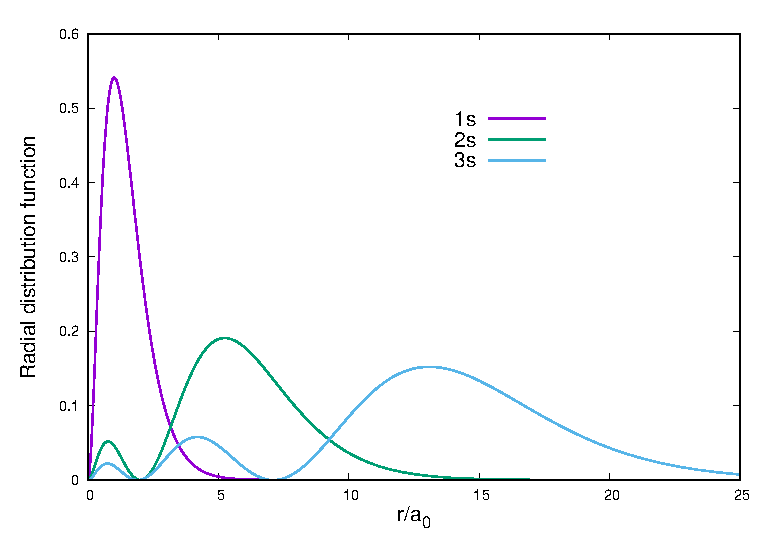
\includegraphics[scale=0.8]{radialdistfuncS.eps}
\caption[Radial distribution function of hydrogenic 1s, 2s, and 3s, electrons]{Radial distribution function of hydrogenic 1s, 2s and 3s, electron. The electron has a higher kinetic energy near the nucleus.}
\label{fig_hydrogen}
\end{figure}
This is the essence of the pseudopotential approximation: the strong core potential is replaced by a pseudopotential, whose shape resembles the potential associated with the all-electron wavefunction outside a certain core radius. In this way both the core states and the nodes (Fig.~\ref{fig_hydrogen}) in the valence wavefunctions are removed. For many metals, the pseudowavefunctions can be represented by a much smaller number of plane waves.
\begin{figure}
\centering
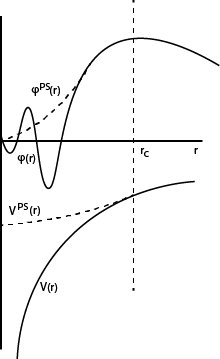
\includegraphics[scale=0.80]{pseudo_figure_01.png}
\caption{Schematic of the replacement of the all-electron wavefunction and core potentials by a pseudo-wavefunction and pseudopotential.}
\end{figure}
\subsection{Basic Phillips--Kleinman Construction}
For a given many-electron Hamiltonian, $\mathcal{H}=\hat{T}+\hat{V}$, where $\hat{T}$ is the kinetic energy operator and $\hat{V}$ is the potential energy operator, the core electron wavefunctions are defined by the time-independent \schrod equation,
\begin{equation}
 \mathcal{H}\ket{\psi_i} = E_i \ket{\psi_i} \quad   (i = 1,\dotsc, n_{\text{core}})
\end{equation}

The valence electron wavefunction similarly can be found by the Hamiltonian
\begin{equation}
\label{eq_val_hamil}
\mathcal{H}\ket{\psi_{\upsilon}} = E_{\upsilon} \ket{\psi_{\upsilon}}
\end{equation}
The valence electron wavefunctions are orthogonal to the core electron wavefunctions $\big(\braket{\psi_{\upsilon}}{\psi_i}=0\big)$, this orthogonality always has to be preserved, even if the core electrons are not treated explicitly. One way to preserve this orthogonality is to write the valence electron wavefunction in a basis set that is orthogonal to the core electrons. The Gram--Schmidt process can be used. Herring~\cite{herring1940new} was the first one to use orthogonalized plane waves (OPWs) (Appendix~\ref{appen_opw}) as basis for the first quantitative calculations of bands. Using this idea, we can orthogonalize any arbitrary basis set $\{\ket{\chi_n}\}$ to the core electron wavefunctions by defining a new basis set $\{\ket{\varrho_n}\}$ via
\begin{equation}
\label{eq_pk}
\ket{\varrho_n} = \ket{\chi_n} - \sum^{n_{\text{core}}}_{i=1} \braket{\psi_i}{\chi_n}\ket{\psi_i}
\end{equation}
Here each of the new basis set, $\{\ket{\varrho_n}\}$, satisfies $\braket{\chi_n}{\psi_i} = 0$ for each $\ket{\psi_i}$. Now we can express the valence electron wavefunction as a linear combination of the new basis sets,
\begin{equation}
\label{eq_val}
\ket{\psi_{\upsilon}} = \sum_n C_n \ket{\varrho_n}. 
\end{equation}
Inserting Eqn.~\eqref{eq_pk} into Eqn.~\eqref{eq_val}, the valence electron wavefunction can be expressed in the following way. The orthogonality condition with the core electrons is still valid,
\begin{equation}
\ket{\psi_{\upsilon}} = \sum_n C_n \left [ \ket{\chi_n} - \sum_{i=1}^{n_{\text{core}}} \ket{\psi_i}\braket{\psi_i}{\chi_n} \right ] = \ket{\phi} - \hat{\Omega}\ket{\phi},
\end{equation}
Here, $\hat{\Omega}$ is a projection operator for the core electron wavefunction
\begin{equation}
\label{eq_projection}
\hat{\Omega} = \sum_{i=n}^{n_{\text{core}}} \dyad{\psi_i}{\psi_i}
\end{equation}
and a new wavefunction which is a linear combination of $\ket{\chi_n}$, sometime designated as pseudo-orbital,
\begin{equation}
\label{eq_pseudoorbital}
\ket{\phi} = \sum_n C_n \ket{\chi_n}
\end{equation}
This technique of representing the valence electron wavefunction in preorthogonalized basis set has been studied and used as a computational tool~\cite{herring1940new}. It took the insight of the Phillips and Kleinman~\cite{phillips1959new}. The new pseudo-orbital satisfies the orthogonality condition, but they also change the Hamiltonian so that the eigenvalues are the same as they would be with the valence electrons. Mathematically, it can be obtained by replacing original valence electron Hamiltonian (Eqn.~\eqref{eq_val_hamil}) with the newly obtained pseudo-wavefunction yields
\begin{equation}
\label{eq_ps_pot}
\mathcal{H}\ket{\psi_{\upsilon}} = \mathcal{H} \left [ \ket{\phi} - \sum_n \ket{\psi_i}\braket{\psi_i}{\phi} \right ] =E_{\upsilon} \left [ \ket{\phi} - \sum_n \ket{\psi_i}\braket{\psi_i}{\phi}  \right ] 
\end{equation}
Rearranging Eqn.~\eqref{eq_ps_pot} provides a new effective Hamiltonian,
\begin{equation}
\label{eq_ps_hamil}
\left [ \mathcal{H} + \sum_n ^{n_{\text{core}}} (E_{\upsilon} - E_i)\ket{\psi_i}\bra{\psi_i}\right ]\ket{\phi} = 
E_{\upsilon}\ket{\phi}
\end{equation}
The above equation has the form of the original valence electron eigenvalue problem (\ref{eq_val_hamil}), but with an extra term for orthogonalization. This extra potential $\Big(V_{n\ell} = \sum_n^{\text{core}} \dyad{\psi_i}{\psi_i}\Big)$, is a non-local operator, and the pseudo-orbital $\bigl(\ket{\phi}\bigr)$ is an eigenstate of the new effective Hamiltonian, $\mathcal{H} + V_{n\ell}$. The new Hamiltonian has an extra potential $V_{n\ell}$, which depends on the angular momentum $\ell$ due to the spherical symmetry. Because of its spherical symmetry, each angular momentum ($\ell$, $m$) combination can be treated separately. The dependence on $\ell$ means that a pseudopotential is a non-local operator, can be written in ``semilocal'' (SL) form:
\begin{equation}
\label{eq_sl}
\hat{V}_{SL} = \sum_{\ell m} \ket{Y_{\ell m}}V_\ell(r)\bra{Y_{\ell m}},
\end{equation}
where $Y_{\ell m}(\theta,\phi) = P_\ell(\cos(\theta))e^{im\theta}$ and $P_l$ is a Legendre polynomial. It is semi-local because it is non local on the angular variables but local in the radial variable.%\footnote{$P_l$ is the Legendre polynomials}


The sophistication and accuracy of pseudopotentials have evolved considerably since the Phillips--Kleinman construction. This development produces many methods of generating pseudopotentials. All of these methods have the following goals: (1) the pseudopotential should be as soft as possible so that it can allow representation of pseudo-wavefunctions with fewer plane waves; (2) transferability has to be maintained, meaning a generated pseudopotential generated to match certain properties should produce other properties accurately; and (3) the pseudo-charge density should reproduce the valence charge density as accurately as possible. 


\subsection{Norm-Conserving Pseudopotentials}
Hamann, Schl\"uter, and Chiang~\cite{hamann1979norm} developed the concept of norm-conservation, which was a first step in fulfilling all the aforementioned requirements. As the exchange--correlation energy of the electronic system depends on the electron density, it is necessary that the real and pseudo wavefunctions be identical outside the core region. In the outer region ($r > r_c$), both functions coincide. Therefore, the total charge density created in the core region $(r < r_c)$ must be the same,
\begin{equation}
\int^{r_{c}}_0 \psi^{\ast}_{ae}(r)\psi_{ae}(r)dr = \int^{r_c}_0 \psi^{\ast}_{ps}(r)\psi_{ps}(r)dr
\end{equation}
\nomenclature{$\psi_{AE}$}{all-electron wavefunction}
\nomenclature{$\psi_{ps}$}{pseudo-wavefunction}
Where $\psi_{ae}(r)$ is the all-electron wavefunction and $\psi_{ps}$ is the pseudo-wavefunction. The logarithmic derivatives of the real and pseudo-wavefunction and their energy derivatives agree in the outer region. These types of pseudopotentials are the most transferable because they are able to reproduce the scattering properties of ions in different chemical environments~\cite{hamann1979norm}. The downside of norm-conserving pseudopotentials is a higher cutoff radius and thus increased memory and CPU requirements. Troullier and Martins~\cite{troullier1991efficient} developed a more effective method to generate norm-conserving pseudopotentials for practical calculations. 

\subsection{Ultrasoft Pseudopotentials (US)}
The norm conservation requirement necessitates a very high of cutoff energy for the plane-wave basis set. In particular, the tightly-bound orbitals have a substantial fraction of their weight inside the core region of the atom. There are some important cases in which it is impossible to construct a pseudopotential that allows a significant reduction of the cutoff energy. Vanderbilt~\cite{vanderbilt1990soft} suggested relaxing the norm conservation criteria in favor of a smoother (\ie,\ softer) pseudopotential. The resulting ultrasoft pseudopotentials are difficult to construct and require extensive testing~\cite{kresse1999ultrasoft}.

\subsection{Projector Augmented Wave Method (PAW)}
The electronic wavefunctions oscillate wildly near the nuclei (Fig.~\ref{fig_hydrogen}) than the valence electrons between the atoms. Expanding the core electrons using plane-wave creates computational challenges. Augmented-wave methods uses the separation of the wavefunctions in two regions to address this issue. The first part is partial wave expansion inside an atom-centered sphere called the augmentation region and a plane wave expansion outside. Both expansions are continuously differentiable at the boundary.

Bl\"ochl~\cite{blochl1994projector} suggested that there is a linear transformation from the all-electron to the pseudo-wavefunctions. The transformation is as follows:
\begin{equation}
\ket{\psi} = \ket{\tilde{\psi}} + \sum_i \left(\ket{\phi_i} - \ket{\tilde{\phi_i}}\right)\braket{\tilde{p_i}}{\tilde{\psi}}
\end{equation}
Here $\phi_i$ are the partial waves within the augmentation regions and $\bra{\tilde{p_i}}$ is a projector that satisfies the condition $\braket{\tilde{p_i}}{\tilde{\phi_j}} = \delta_{ij}$. The tilde quantities are related the pseudo representation. Kresse and Joubert~\cite{kresse1999ultrasoft} showed a connection between PAW and ulstrasoft pesudopotential (US-pp) and how the PAW method can be implemented into existing code.

\begin{comment}
\section{Defects in Solids}
Structural discontinuities and localized regions of disorder are invariably present in real solids. This heterogeneity can exist in both microscopic and macroscopic scales. To understand diffusion in solids, we need to understand the so called `perfect crystal'. A perfect crystal has a rigid stoichiometry in which a simple proportion of a few atomic species are bound together in an finite, and regular array. The lattice is usually regarded as the repetitive entity that defines the translational symmetry in the crystal structure. Even with the presence of \textit{imperfection}, the crystal surface, the translational invariance is destroyed; it effects, however, are neglected by the definition of the `bulk' properties. Other defects are almost inevitably present in the crystal.
%\subsection{Lattice Vacancy}

Of the various lattice defects the vacancy is the only species that is ever present appreciable concentration in thermal equilibrium and increases exponentially with temperature.
To understand the thermodynamics of vacancy formation, lets consider a set of $N$ atoms in $N$ lattice site in the crystal. The free energy of the perfect crystal will be $G_0$. If we remove $n$ atoms from the crystal and place them on the surface we have therefore formed an vacancy sites. Each of these vacancies will be associated with an enthalpy of formation $\Delta H_V$ and an excess entropy $\Delta S_V$. There will be a configurational or mixing entropy change associated with formation of $n$ vacancies given by
\begin{equation}
\Delta S_c = k_B \ln\mathcal{W}
\end{equation}
\nomenclature{$\mathcal{W}$}{number of different combination of atoms and vacancies}
here $\mathcal{W}$ is the number of different configuration of atoms, and $k_B$ is the Boltzmann's constant. With n vacancies and $N$ atoms distributed among $(N+n)$ sites, the number of possible different configuration is :
\begin{align}
\begin{split}
\mathcal{W} & = \frac{(N+n)!}{n!} \\
\Delta S_c & = k_B\ln \frac{(N+n)!}{N!n!}
\end{split}
\end{align}
\nomenclature{$S_c$}{configurational entropy due to the presence of vacancy}
\nomenclature{$S_V$}{entropy of vacancy formation}
Using the Stirling's approximation ($\ln\ (N!)=N\ \ln N - N$, for $(N\rightarrow \infty)$) the above equation becomes:
\begin{equation}\label{eq_sc}
\Delta S_c = -k_B \left [ N\ln\ \frac{N}{(N+n)} + n\ln\ \frac{n}{(N+n)}   \right ]
\end{equation}
Therefore the change in free energy would be
\begin{equation}
\Delta G = G - G_0 = n \Delta H_V -  T \Delta S = n \Delta H_V - T(\Delta S_c + n \Delta S_V)
\end{equation}
Using Eqn.~\ref{eq_sc} the above equation becomes
\begin{equation}\label{eq_free}
\Delta G = n \Delta H_V + k_B\left (N\ln\ \frac{N}{(N+n)} + n\ln\ \frac{n}{(N+n)}\right ) - nT\Delta S_V   
\end{equation}
The equilibrium vacancy concentration happens when the free energy~(\ref{eq_free}) is minimized with respect to vacancy $n$. Thus we find 
\begin{equation}
\frac{\partial G}{\partial n}  = \Delta H_V - T\Delta S_V + k_{B}T\ln\ \frac{n}{(N+n)} = 0
\end{equation}
Upon rearrangement,
\begin{equation}
\frac{n}{(N+n)} = e^{\left (\frac{\Delta S_V}{k_B} \right )} e^{\left (-\frac{\Delta H_V}{k_B T}  \right)}
\end{equation}
Since $n\lll N$, the above equation can be rearranged as
\begin{equation}
\ln \frac{n}{(N+n)} \backsimeq \ln \frac{n}{N} = - \frac{\Delta H_V - T\Delta S_V}{k_BT}
\end{equation}
The fractional concentration of vacancy may be expressed as follows
\begin{equation}
C_v = \frac{n}{N} = e^{\left(- \frac{\Delta H_V - T\Delta S_V}{k_B T} \right )}
\end{equation}
\nomenclature{$C_v$}{vacancy concentration}
At atmospheric pressure the formation enthalpy is identical to formation energy ($E_{\Box}^f$). The concentration of defects at any temperature can be estimated as 
\begin{equation}\label{eq_vacconc}
C_v = e^{\left(\Delta S_V/k_B \right)} e^{\left(-E_{\Box}^f/k_BT  \right )}
\end{equation}


\section{Atomic Diffusion in Solids}
In solid, the impurities or host atom can move from one equilibrium site to another. For simplicity, lets assume the solute's minimum energy location is the bcc lattice site. As the atom moves from center to any direction, it encounters an increase in potential energy. If the solute atom gains enough energy, it can move out of one lattice site to the nearest vacancy. This act is the diffusive jump. The magnitude of the barrier that the migrating atom needs to overcome from one equilibrium position to the next equilibrium position can be calculated by computing the potential energy of the system comprising the solute atom along the jump. The energy is a minimum when the solute is in an equilibrium position and attains a maximum halfway between the equilibrium sites. The difference in potential energy between the equilibrium position and the maximum, or saddle point, is the activation/migration  energy for diffusion, $E_{\text{mig}}$,
\begin{equation}
E_{\text{mig}}= U\ (\text{saddle point}) - U\ (\text{equilibrium site})
\end{equation}
An atom in saddle point is also said to be in the activated state. The solute atom stays in the equilibrium or local minimum, simply oscillates. The frequency of the oscillation can be calculated from the curvature of the potential energy at equilibrium position using the following relation:
\begin{equation}
\nu = \frac{1}{2\pi} \left (\frac{1}{m}\frac{d^2U}{dx^2} \right )_{x=x_{eq}}^{\frac{1}{2}}
\end{equation}
\nomenclature{$\nu$}{vibrational frequency of an atom in solid}
If the solute atom acquires enough energy greater or equal to the barrier $E^{\text{mig}}$, results in a diffusive jump from one equilibrium site to another. The frequency with which an atom jumps to a nearby site is denoted by $\nu$. This jump frequency can be estimated by transition state theory (TST), first proposed by H. Eyring in 1930s. It was first proposed to explain the kinetics of homogeneous gas phase reaction. This theory, however can be used to explain other rate process including diffusion in solids. The fundamental assumption of TST is that, in any rate process a barrier must be overcome by the moving species for the elementary step to occur. The atom at the top of the barrier is called activated state. It is also assumed that the activated sate is also a thermodynamic state and can be described by partition function. The activated state is treated as any other other type of defect in the crystal. 

\begin{figure}
\centering
\includegraphics[scale=0.6]{sol-vac}
\caption{Schematic of an impurity atom in a BCC crystal jumping from center to nearest vacancy.}
\end{figure}

\begin{figure}
\centering
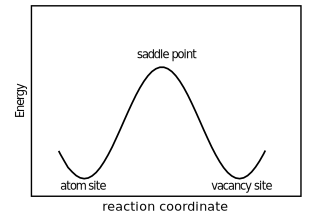
\includegraphics[scale=1.3]{tst-fig}
\caption{Illustration of the energy barrier at the saddle point between the jumping atom site and the neighboring site.}
\label{fig:tst}
\end{figure}

The ratio of the number of diffusing atom in lattice site (initial state) $N_{\text{IS}}$, to the number of diffusing atoms in the transition state , $N_{\text{TS}}$ is given by
\begin{equation}\label{eq:tstratio}
\frac{N_{\text{TS}}}{N_{\text{IS}}} \approx \frac{Q_{\text{TS}}}{Q_{\text{IS}}} exp\ \left(-\frac{E_0}{k_BT}  \right)
\end{equation}
Here, the partition function, $Q_{\text{TS/IS}}$, can be expressed into its vibrational, rotational and translational components.
\begin{equation}
Q = q_{\text{tr}}\ q_{\text{rot}}\ q_{\text{vib}}
\end{equation}

The vibrational part of the partition function  is different from the initial state (equilibrium site). Since one degree of freedom is no longer a vibration, the motion along the minimum energy path is more like a translation and has a lower frequency than other atoms. Lets call this mode's vibration as $\nu^{\ddagger}$. The vibrational partitional function can be approximated as follows:
\begin{equation}
q_{\nu}^{\ddagger} = \frac{e^{h\nu^{\ddagger}/2k_BT}}{1 - e^{-h\nu^{\ddagger}/2k_BT}} \approx \frac{e^{h\nu^{\ddagger}/2k_BT}}{1 - (1-h\nu^{\ddagger}/k_BT + \frac{1}{2}(h\nu^{\ddagger}/k_BT)^2 + \dots)} = \frac{k_BT}{h\nu^{\ddagger}} e^{-h\nu^{\ddagger}/2k_BT}
\end{equation}
Here, the term $ e^{-h\nu^{\ddagger}/2k_BT}$ can be considered as contribution from the zero point energy. Introducing the new addition to the partition function, the equilibrium ratio becomes
\begin{equation}
\frac{N_{\text{TS}}}{N_{\text{IS}}} \approx \frac{k_BT}{h\nu^{\ddagger}} \frac{Q_{\text{TS}}^{\dagger}}{Q_{\text{IS}}} e^{-\frac{E_A}{k_BT}}
\end{equation}
here $E_A = E_0 + \epsilon_0$, $\epsilon_0$ is the is the zero point energy. $Q^{\dagger}$ is the partition function at the saddle point, $\nu^{\ddagger}$ is the frequency at the saddle point. The decomposing rate ($\nu$) con be calculated as follows:
\begin{equation}\label{eq_migfreq}
\nu = \nu^{\ddagger} N_{\text{TS}} = \frac{k_BT}{h} \frac{Q_{\text{TS}}^{\dagger}}{Q_{\text{IS}}} e^{-\frac{E_A}{k_BT}}
\end{equation}
Here the terms, $\frac{k_BT}{h} \frac{Q^{\dagger}_{\text{TS}}}{Q_{\text{IS}}} = \nu_0$, is the so-called attempt frequency, the pre-exponential or simply the prefactor. The second factor $e^{-\frac{E_A}{k_BT}}$ is called the Boltzmann factor. It is given by the activatin energy $E_A$, the Botzmann constant $k_B$, and the temperature, $T$. The pre-exponential factor can be written as:
\begin{equation}\label{eq_entrp}
\nu_0 = \frac{k_BT}{h}\ e^{-\frac{S_A}{k_B}}
\end{equation} 
Here the term, $S_A$, is the so called entropy of activation which is defined as, $S_A = k_B\ln \left( \frac{\nu_0 h}{k_B T} \right )$. The term, $\frac{k_BT}{h} = \num{6e12} s^{-1}$.

\subsection*{Jump Frequency}
The jump frequency ($\Lambda$) is the total jumps per second for an atom. It is proportional to the number of available site nearby ($\beta$) (nearest neighbor), and the probability of having a vacancy in the nearest neighbor site ($P_v$), the frequency ($\nu$)at which an atm jumps to a particular site. Thus, the jump frequency can be calculated as follows:
\begin{equation}\label{eq_jmp}
\Lambda = \beta P_v \nu
\end{equation}
\nomenclature{$\Lambda$}{jump frequency}
\nomenclature{$\beta$}{number of available site in nearest neighbor site}
\nomenclature{$P_v$}{probability of having a vacancy in the nearest neighbor site}
For bcc crystal the number of available site is $6$, the probability of a nearby vacancy can be calculated from Eq.~\eqref{eq_vacconc}, and atomic jump frequency is from Eq.~\eqref{eq_migfreq}. We can use all these microscopic properties and use Einstein formula~\cite{olander1976,was2016} to approximate a macroscopic diffusion parameter, D. According to Einstein formula the diffusion parameter can be formulated using the atomic property $\lambda$, and $\Lambda$,
\begin{equation}\label{eq_ein}
D = \frac{1}{6}\lambda^2 \Lambda
\end{equation}
\nomenclature{$\lambda$}{mean jump distance}
Here $\lambda$ is the jump distance which usually represented in terms of lattice parameter ($=Ca_0$). Using Eq.~\eqref{eq_jmp}, the diffusion parameter becomes:
\begin{equation}
D = \frac{1}{6} \beta C^2 P_v a_0^2 \nu 
\end{equation}
Which is usually written as following:
\begin{equation}
D = \alpha a_0^2 P_v \nu
\end{equation}
Here the term $1/6 \beta C^2$ is represented by a single parameter, $\alpha$, which is property of the crystal. If the vacancy motion is random, then $P_v = C_v$. With the help of Eqn.~\eqref{eq_vacconc}, Eqn.~\eqref{eq_entrp} and Eqn.~\eqref{eq_migfreq}
\begin{equation}\label{eq_slfdif}
D = \left( \frac{k_BT}{h}\right )\alpha a_0 e^{(\Delta S_v + S_a)/k_B}\ e^{(-E_{\Box}^f - E_A)/(k_BT)}
\end{equation}
In the above equation we have combined the entropic contribution of vacancy formation ($\Delta S_v$) and migration ($S_a$), and the enthalipic contribution of vacancy formation ($E_{\Box}^f$) and migration ($E_A$). Eqn.~\eqref{eq_slfdif} is usually used to approximate the vacancy self-diffusion coefficient. The entropic contribution is often ignored because of its very low value (\ie\@ $e^{S/k_B} \approx 1$). The vacancy formation and migration  energy are however play a pivotal role in the diffusion atoms inside the solid matrix. Atomistic methods such as density functional theory or molecular dynamics are usually used to determine these values. In this dissertation we have used supercell approach on DFT to approximate the vacancy formation energy ($E_{\Box}^f$). Nudged elastic band method (NEB)~\cite{henkelman2000climbing, henkelman2000improved} is used to find the saddle point and to determine the activation energy.

\end{comment}



\newpage
\bibliographystyle{apsrev4-2}
\bibliography{abbreviated,final}
%\bibliography{abbreviated,other}
